\PassOptionsToPackage{unicode=true}{hyperref} % options for packages loaded elsewhere
\PassOptionsToPackage{hyphens}{url}
%
\documentclass[]{scrartcl}
\usepackage{lmodern}
\usepackage{amssymb,amsmath}
\usepackage{ifxetex,ifluatex}
\usepackage{fixltx2e} % provides \textsubscript
\ifnum 0\ifxetex 1\fi\ifluatex 1\fi=0 % if pdftex
  \usepackage[T1]{fontenc}
  \usepackage[utf8]{inputenc}
  \usepackage{textcomp} % provides euro and other symbols
\else % if luatex or xelatex
  \usepackage{unicode-math}
  \defaultfontfeatures{Ligatures=TeX,Scale=MatchLowercase}
\fi
% use upquote if available, for straight quotes in verbatim environments
\IfFileExists{upquote.sty}{\usepackage{upquote}}{}
% use microtype if available
\IfFileExists{microtype.sty}{%
\usepackage[]{microtype}
\UseMicrotypeSet[protrusion]{basicmath} % disable protrusion for tt fonts
}{}
\IfFileExists{parskip.sty}{%
\usepackage{parskip}
}{% else
\setlength{\parindent}{0pt}
\setlength{\parskip}{6pt plus 2pt minus 1pt}
}
\usepackage{hyperref}
\hypersetup{
            pdftitle={Devoir Maison de mathématiques},
            pdfauthor={Oscar Plaisant},
            pdfborder={0 0 0},
            breaklinks=true}
\urlstyle{same}  % don't use monospace font for urls
\setlength{\emergencystretch}{3em}  % prevent overfull lines
\providecommand{\tightlist}{%
  \setlength{\itemsep}{0pt}\setlength{\parskip}{0pt}}
\setcounter{secnumdepth}{0}
% Redefines (sub)paragraphs to behave more like sections
\ifx\paragraph\undefined\else
\let\oldparagraph\paragraph
\renewcommand{\paragraph}[1]{\oldparagraph{#1}\mbox{}}
\fi
\ifx\subparagraph\undefined\else
\let\oldsubparagraph\subparagraph
\renewcommand{\subparagraph}[1]{\oldsubparagraph{#1}\mbox{}}
\fi

% set default figure placement to htbp
\makeatletter
\def\fps@figure{htbp}
\makeatother

\usepackage[utf8]{inputenc}
\usepackage[T1]{fontenc}
\usepackage[french]{babel}

\usepackage[left=1.2cm, right=1.2cm, top=2cm, bottom=2.5cm]{geometry}

\usepackage{amsmath, amsfonts, amssymb}

\usepackage{lastpage}

\usepackage{xcolor}
\usepackage{enumitem}
\usepackage{fancyhdr}
\usepackage{sectsty}
\usepackage{graphicx}
\usepackage{euler}

\pagestyle{fancy}

\renewcommand{\headrulewidth}{0pt}
\fancyhead[L]{}
\fancyhead[C]{}
\fancyhead[R]{}

\renewcommand{\footrulewidth}{1pt}
\fancyfoot[L]{Antonin\;Peronnet,\;Benoit\;Leroux,\;Oscar\;Plaisant}
\fancyfoot[C]{\thepage/\pageref{LastPage}}
\fancyfoot[R]{\.\.\text{DM N}$^\circ3$}

\renewcommand{\frac}[2]{\dfrac{#1}{#2}}

\sectionfont{\Huge}
\subsectionfont{\huge}
\subsubsectionfont{\Large}
\paragraphfont{\large}

\title{\huge Devoir Maison de mathématiques}
\author{Oscar Plaisant}
\date{}

\begin{document}
\maketitle

\hypertarget{exercice-1}{%
\section{Exercice 1 :}\label{exercice-1}}

\(u_0 = 3\)

\(u_1 = 6\)

\(u_{n+2} = \dfrac{5}{4}u_{n+1} -\dfrac{1}{4}u_n\)

\hypertarget{partie-a}{%
\subsection{Partie A}\label{partie-a}}

\hypertarget{donner-une-formule-qui-saisie-dans-la-cellule-b4-puis-recopiuxe9e-vers-le-bas-permet-dobtenir-les-valeurs-de-la-suite-u_n-dans-la-colonne-b.}{%
\subsubsection{\texorpdfstring{1. Donner une formule qui, saisie dans la
cellule B4, puis recopiée vers le bas, permet d'obtenir les valeurs de
la suite \((u_n)\) dans la colonne
B.}{1. Donner une formule qui, saisie dans la cellule B4, puis recopiée vers le bas, permet d'obtenir les valeurs de la suite (u\_n) dans la colonne B.}}\label{donner-une-formule-qui-saisie-dans-la-cellule-b4-puis-recopiuxe9e-vers-le-bas-permet-dobtenir-les-valeurs-de-la-suite-u_n-dans-la-colonne-b.}}

La formule est ``=(5*B3/4) + (B2/4)''

\hypertarget{recopier-et-compluxe9ter-le-tableau-ci-dessus.-on-donnera-des-valeurs-approchuxe9es-uxe0-10---3-pruxe8s-deun-pour-n-allant-de-2-uxe0-5.}{%
\subsubsection{\texorpdfstring{2. Recopier et compléter le tableau
ci-dessus. On donnera des valeurs approchées à 10 - 3 près deun pour
\(n\) allant de 2 à
5.}{2. Recopier et compléter le tableau ci-dessus. On donnera des valeurs approchées à 10 - 3 près deun pour n allant de 2 à 5.}}\label{recopier-et-compluxe9ter-le-tableau-ci-dessus.-on-donnera-des-valeurs-approchuxe9es-uxe0-10---3-pruxe8s-deun-pour-n-allant-de-2-uxe0-5.}}

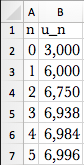
\includegraphics[scale=0.5]{images/tableur.png}

\hypertarget{que-peut-on-conjecturer-uxe0-propose-de-la-convergence-de-la-suite-u_n}{%
\subsubsection{\texorpdfstring{3. Que peut-on conjecturer à propose de
la convergence de la suite \((u_n)\)
?}{3. Que peut-on conjecturer à propose de la convergence de la suite (u\_n) ?}}\label{que-peut-on-conjecturer-uxe0-propose-de-la-convergence-de-la-suite-u_n}}

On peut conjecturer que la suite diverge vers \(+\infty\)

\hypertarget{partie-b}{%
\subsection{Partie B}\label{partie-b}}

\hypertarget{section}{%
\subsubsection{1.}\label{section}}

\hypertarget{a-duxe9montrer-que-v_n-est-une-suite-constante}{%
\paragraph{\texorpdfstring{a) Démontrer que \((v_n)\) est une suite
constante}{a) Démontrer que (v\_n) est une suite constante}}\label{a-duxe9montrer-que-v_n-est-une-suite-constante}}

\[
\begin{array}{rcl}
    v_n = u_{n+1} - \dfrac{1}{4}u_n & \iff & v_{n+1} = u_{n+2} + \dfrac{1}{4}u_{n+1}\\
        &\iff& v_{n+1} = \left(\dfrac{5}{4}u_{n+1} - \dfrac{1}{4}u_n\right) - \dfrac{1}{4}u_{n+1}\\
        &\iff& v_{n+1} = u_{n+1} - \dfrac{1}{4}u_{n+1}\\
        &\iff& v_{n+1} = v_n
\end{array}
\] Donc, la suite \((v_n)\) est constante. \#\#\#\# b) En déduire que,
pour tout \(n\in\mathbb{N}, u_{n+1} = \dfrac{1}{4}u_n + \dfrac{21}{4}\)

On sait que \[
\begin{array}{rcl}
    u_{n+1} &=& v_n + \dfrac{1}{4}u_n\\
            &=& v_0 + \dfrac{1}{4}u_n\\
            &=& \dfrac{21}{4} + \dfrac{1}{4}u_n\\ 
\end{array}
\]

\hypertarget{section-1}{%
\subsubsection{2.}\label{section-1}}

\hypertarget{a-en-utilisant-le-ruxe9sultat-de-la-question-1.b-montrer-par-ruxe9currence-que-forall-ninmathbbn-u_nleq-u_n1leq-15}{%
\paragraph{\texorpdfstring{a) En utilisant le résultat de la question
\textbf{1.b)}, montrer par récurrence que
\(\forall n\in\mathbb{N}, u_n\leq u_{n+1}\leq 15\)\textbackslash{}}{a) En utilisant le résultat de la question 1.b), montrer par récurrence que \textbackslash{}forall n\textbackslash{}in\textbackslash{}mathbb\{N\}, u\_n\textbackslash{}leq u\_\{n+1\}\textbackslash{}leq 15\textbackslash{}}}\label{a-en-utilisant-le-ruxe9sultat-de-la-question-1.b-montrer-par-ruxe9currence-que-forall-ninmathbbn-u_nleq-u_n1leq-15}}

On pose \(P\), la proposition : \(P_n \iff u_n\leq u_{n+1}\leq 15\)

\hypertarget{initialisation}{%
\subparagraph{Initialisation}\label{initialisation}}

\(P_0 \iff u_0 \leq u_1 \leq 15 \iff 3 \leq 6\leq 15\)

Donc, \(P_0\) est vraie.

\hypertarget{huxe9ruxe9dituxe9}{%
\subparagraph{Hérédité}\label{huxe9ruxe9dituxe9}}

On cherche à montrer que
\(\forall n\in\mathbb{N}, P_n\implies P_{n+1}\).

\[
\begin{array}{rcl}
    P_n &\iff& u_n \leq u_{n+1}\leq 15\\[2ex]
        &\iff& \dfrac{1}{4}u_n \leq \dfrac{1}{4}u_{n+1} \leq \dfrac{15}{4}\\[2ex]
        &\iff& \dfrac{1}{4}u_n + \dfrac{21}{4}u_n \leq \dfrac{1}{4}u_{n+1} + \dfrac{21}{4} \leq \dfrac{15}{4} + \dfrac{21}{4}\\[2ex]
        &\iff& u_{n+1} \leq u_{n+2} \leq 9\\[2ex]
        &\implies& u_{n+1} \leq u_{n+2} \leq 15
\end{array}
\]

On à donc bien \(P_n \implies P_{n+1}\)

\hypertarget{ruxe9currence}{%
\subparagraph{Récurrence}\label{ruxe9currence}}

puisque \(P_0 \wedge \forall n\in\mathbb{N}, P_n\implies P_{n+1}\), on
sait que \(\forall n\in\mathbb{N}, P_n\) b) En déduire que la suite
\((u_n)\) est une suite convergente.

La suite \((u_n)\) est strictement croissante et majorée par 15, on peut
donc dire qu'elle converge.

\hypertarget{section-2}{%
\subsubsection{3.}\label{section-2}}

\hypertarget{a-duxe9montrer-que-w_n-est-une-suite-guxe9omuxe9trique-dont-on-pruxe9cisera-le-premier-terme-et-la-raison}{%
\paragraph{\texorpdfstring{a) Démontrer que \((w_n)\) est une suite
géométrique dont on précisera le premier terme et la
raison}{a) Démontrer que (w\_n) est une suite géométrique dont on précisera le premier terme et la raison}}\label{a-duxe9montrer-que-w_n-est-une-suite-guxe9omuxe9trique-dont-on-pruxe9cisera-le-premier-terme-et-la-raison}}

On sait que :

\(w_n = u_n - 7\)

On peut donc en déduire que :

\(w_0=u_0-7=3-7=-4\)

Et que :

\[
\begin{array}{rcl}
    w_{n+1} &=& u_{n+1} - 7\\
            &=& \dfrac{u_n}{4} + \dfrac{21}{4} - \dfrac{28}{4}\\
            &=& \dfrac{u_n - 7}{4}\\
    w_{n+1} &=& \dfrac{1}{4}w_n
\end{array}
\]

On à donc :

\(\left\{\begin{array}{rcl}w_0 &=& -4\\w_{n+1} &=& \dfrac{1}{4}w_n\end{array}\right.\)

On peut donc dire que la suite \((w_n)\) est une suite de premier terme
-4 et de raison \(\dfrac{1}{4}\).

\hypertarget{b-en-duxe9duire-que-forall-ninmathbbn-u_n-7--leftdfrac14rightn-1}{%
\paragraph{\texorpdfstring{b) En déduire que
\(\forall n\in\mathbb{N}, u_n = 7 -\left(\dfrac{1}{4}\right)^{n-1}\)}{b) En déduire que \textbackslash{}forall n\textbackslash{}in\textbackslash{}mathbb\{N\}, u\_n = 7 -\textbackslash{}left(\textbackslash{}dfrac\{1\}\{4\}\textbackslash{}right)\^{}\{n-1\}}}\label{b-en-duxe9duire-que-forall-ninmathbbn-u_n-7--leftdfrac14rightn-1}}

On sait que \((w_n)\) est la suite géométrique de raison
\(\dfrac{1}{4}\) et de premier terme -4. On peut donc dire que
\(w_n = -4\left(\dfrac{1}{4}\right)^{n} =-\left(\dfrac{1}{4}\right)^{n-1}\)

On sait également que \(w_n = u_n - 7\), soit que \(u_n = 7 + w_n\).

On peut donc dire que
\(w_n = u_n - 7\iff w_n = 7 -\left(\dfrac{1}{4}\right)^{n-1}\)

\hypertarget{c-calculer-la-limite-de-la-suite-u_n}{%
\paragraph{\texorpdfstring{c) calculer la limite de la suite
\((u_n)\)}{c) calculer la limite de la suite (u\_n)}}\label{c-calculer-la-limite-de-la-suite-u_n}}

On sait que \(u_n = 7 - \left(\dfrac{1}{4}\right)^{n-1}\). On cherche
donc à calculer
\(\lim_{n\rightarrow +\infty}\left(7 - \left(\dfrac{1}{4}\right)^{n-1}\right)\)
:

\[\newcommand{\disp}{\displaystyle}
\begin{array}{rcl}
    \disp\lim_{n\rightarrow +\infty}\left(u_n\right) &=& \disp\lim_{n\rightarrow +\infty}\left(7 - \left(\dfrac{1}{4}\right)^{n-1}\right)\\[2ex]
        &=& \disp\lim_{n\rightarrow +\infty}(7) - \lim_{n\rightarrow +\infty}\left(\left(\dfrac{1}{4}\right)^{n - 1}\right)\\[2ex]
        &&\text{Or, }\;\;\dfrac{1}{4}\in ]-1; 1[\;\;\text{ Donc :}\\[2ex]
        &=& 7 - 0\\
        &=& 7
\end{array}
\]

\end{document}
